\documentclass[12pt,a4paper]{article}
\usepackage[T2A]{fontenc}
\usepackage[russian]{babel}
\usepackage[utf8]{inputenc}
\ifx\pdfoutput\undefined
	\usepackage{graphicx}
\else
	\usepackage[pdftex]{graphicx}
	\usepackage{epstopdf}
\fi
\usepackage{amssymb}
\usepackage{amsmath}
\usepackage[font=normalsize,labelfont=bf]{caption}
\usepackage[unicode=true, hypertexnames=false]{hyperref}
\usepackage{afterpage}
\hypersetup{
		pdftitle={Богданов Д.А., “Численное исследование течения в фильтре-циклоне”, 2012},
    colorlinks,
    citecolor=black,
    filecolor=black,
    linkcolor=black,
    urlcolor=black
}
\oddsidemargin=0pt
\textwidth=155mm
\title{Численное исследование течения в фильтре-циклоне}
\author{Дмитрий Богданов}
\date{}
\renewcommand\normalsize{\fontsize{14pt}{24pt}\selectfont}
\begin{document}
\begin{titlepage}
	\begin{center}
		\small{МИНИСТЕРСТВО ОБРАЗОВАНИЯ И НАУКИ \\ РОССИЙСКОЙ ФЕДЕРАЦИИ \\
Санкт-Петербургский государственный политехнический университет \\
Физико-механический факультет \\
Кафедра гидроаэродинамики}\\
		\vspace{0.05\textheight}
	\end{center}
	\begin{flushright}
		\normalsize
			Диссертация допущена к защите \\
			Зав. кафедрой, проф., д.ф-м.н.\\
			\underline{\hspace{7em}} Е.М. Смирнов \\
			"\underline{\hspace{2em}}" \underline{\hspace{9em}} 2012г. \\
	\end{flushright}
	\begin{center}
		\vspace{0.1\textheight}
		\large{Численное исследование течения в фильтре-циклоне}\\
		\vspace{0.01\textheight}
		\normalsize
		\textsc{Диссертация на соискание ученой степени магистра по направлению 010600 – Прикладные математика и физика}
		\vspace{0.25\textheight}
	\end{center}
	\begin{minipage}{0.48\textwidth}
		\begin{flushleft}
			Выполнил студент гр. 6054/11\\
			Руководитель, к.ф.-м.н., доц.\\
		\end{flushleft}
	\end{minipage}
	\begin{minipage}{0.5\textwidth}
		\begin{flushright}
			Богданов Д.А. \\
			Поняев С.А. \\
		\end{flushright}
	\end{minipage}
	\vspace{0.1\textheight}
	\begin{center}
		Санкт-Петербург \\
		\the\year
	\end{center}
\end{titlepage}
\newpage

\tableofcontents
\newpage
\section*{Введение}
\addcontentsline{toc}{section}{Введение}
	\subsection*{Актуальность проблемы}
	\addcontentsline{toc}{subsection}{Актуальность проблемы}
		\hspace{1em} 	Задача очищения атмосферного воздуха от загрязняющих выбросов промышленных предприятий достаточно актуальна. Выбросы от стационарных источников вредных веществ в атмосферу городов и населенных пунктов, расположенных на территории северо-западного федерального округа,  по данным Росстата за 2007 год,  составили 2319000 тонн, в том числе твёрдых -- 289400 тонн \cite{emissionInfoRussian}. В некоторых отраслях промышленности доля выбросов пыли в атмосферу достигает 15\% от общего числа получаемого продукта. Так, при изготовлении одной тонны цемента в воздух выбрасывается $\approx 160$ кг цементной пыли \cite{emissionInfoEurope}.
		\begin{figure}[ht]
			\begin{minipage}{0.46\linewidth}
				\vspace{-1em}
				Динамика изменения объёма выбросов твёрдых вредных веществ в атмосферу \textit{(рисунок \ref{figure:atmosphereDynamic})} имеет тенденцию к росту, что говорит о том, что решение проблемы инженерной защиты воздуха от вредных веществ останется актуальной и в ближайшем будущем. 
			\end{minipage}
			\hspace{0.01\linewidth}
			\begin{minipage}{0.48\linewidth}
				\centering
				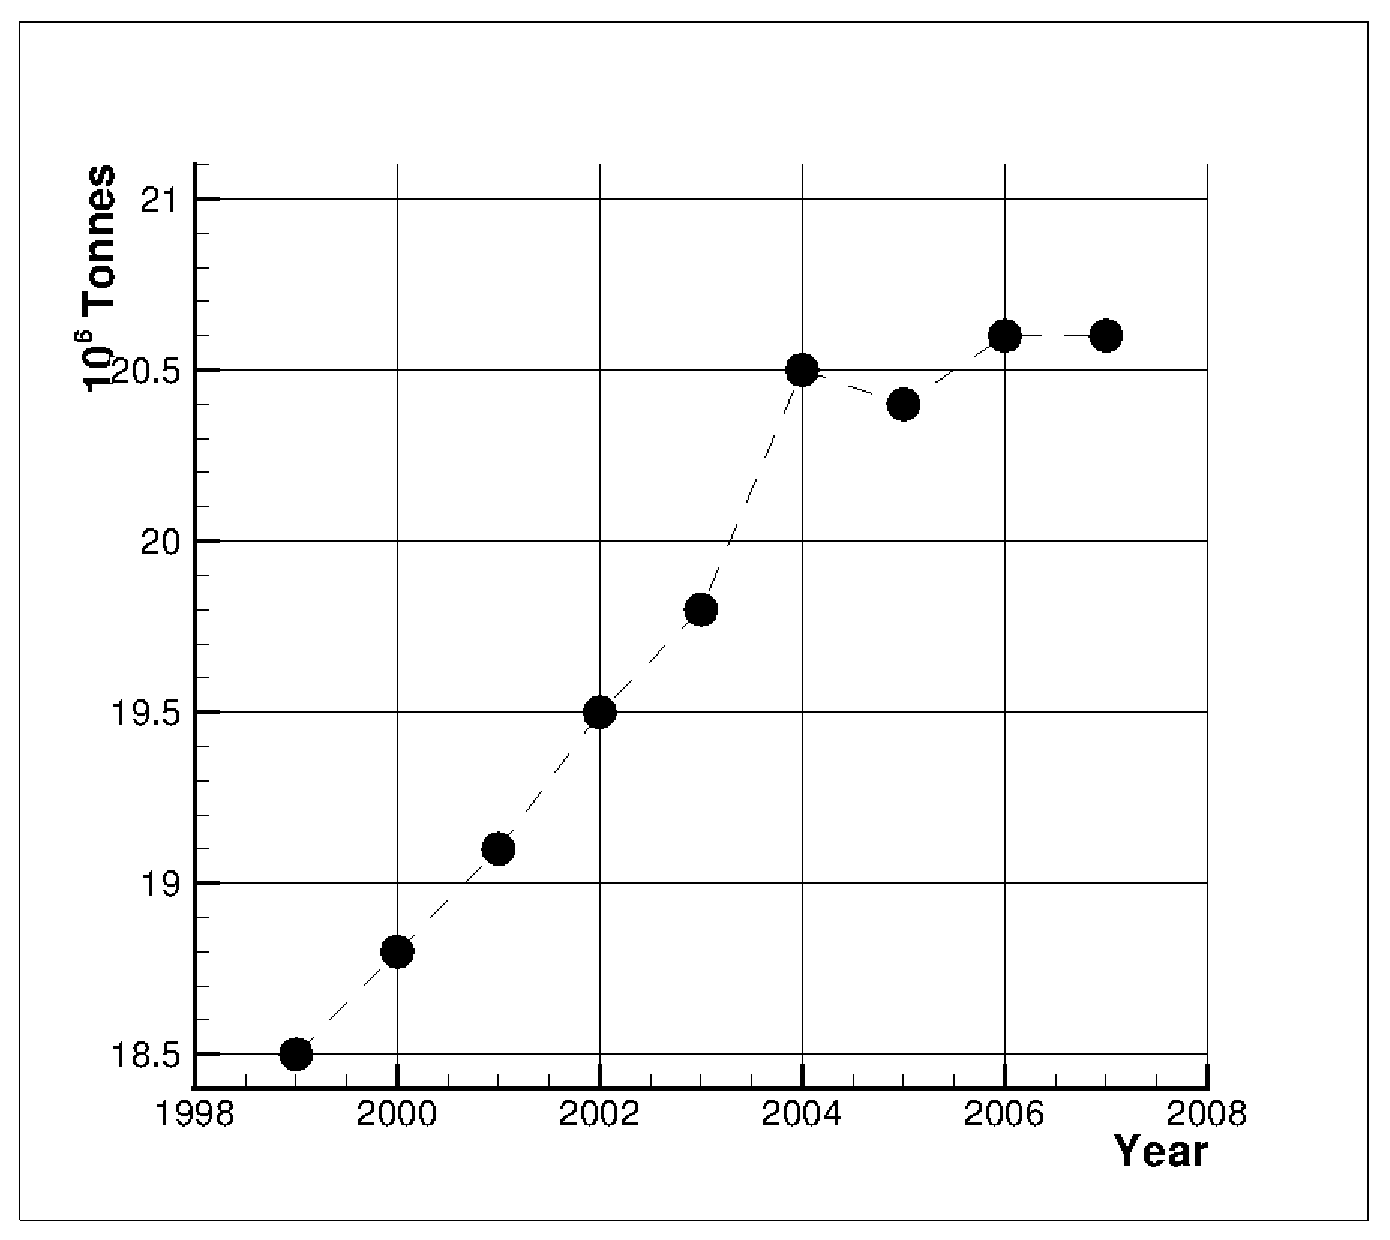
\includegraphics[scale=0.26]{atmosphereDynamic1}
				\caption{Динамика выбросов твёрдых веществ в атмосферу \cite{emissionInfoRussian}}
				\label{figure:atmosphereDynamic}
			\end{minipage}
		\end{figure}
		\vspace{-1em}
	
		Для очищения воздуха от твёрдых примесей широкое распространение получили фильтры типа циклон. Циклон представляет собой инерционный пылеуловитель, в котором выделение частиц из воздушной среды происходит, в основном, под действием центробежной силы, возникающей при вращении воздушного потока в корпусе аппарата.
	
		Запылённый воздух входит в циклон через тангенциальный патрубок и, приобретая вращательное движение, опускается винтообразно вниз вдоль внутренних стенок цилиндра и конуса. Небольшая часть этого потока, в котором сконцентрированы пылевые частицы, движется в непосредственной близости от стенок циклона и поступает через пылеотводящее отверстие в пылесборный бункер, где происходит осаждение и накопление пылевых частиц.
	
		В центральной зоне циклона воздушный поток, освобождённый от пыли, поднимается винтообразно вверх и удаляется через выхлопную трубу наружу.
	
		Вследствие вращательного движения воздушного потока в центральной зоне циклона (в конусе, выхлопной трубе и пылесборном бункере) наблюдается пониженное давление.\cite{instructions}
	
		В силу высокой степени закрученности потока, необходимо введение поправок в модели турбулентности для учёта кривизны линий тока. Кроме того, учитывая высокую концентрацию частиц в потоке, в инженерных расчётах необходимо учитывать не только влияние потока на частицы, но также и обратное влияние частиц на поток.
	%Актуальность проблемы
	\subsection*{Цели работы}
	\addcontentsline{toc}{subsection}{Цели работы}
		\begin{enumerate}
			\item Реализация $k-\omega-SST$ модели турбулентности с поправкой на кривизну линий тока при помощи открытой интегрируемой платформы для численного моделирования задач механики сплошных сред OpenFOAM.
			\item Реализация с использованием OpenFOAM солвера, имеющего в основе модель идеального газа и учитывающего при этом обратное влияние частиц на поток.
			\item Численное моделирование циклона с учётом обратного влияния частиц на поток и поправки на кривизну линий тока к генерации турбулентности.
		\end{enumerate}
	%Цели работы
%Введение

\newpage
<<<<<<< HEAD
%!TEX root = Dissertation.tex
\newpage
=======
>>>>>>> pif/master
\section{Численное моделирование}
	\subsection{Уравнения движения}
		\subparagraph{Уравнение баланса массы\\}
			\begin{equation}
				\frac{\partial \rho}{\partial t} + \frac{\partial}{\partial x_i}(\rho u_i) = 0
			\end{equation}
		\subparagraph{Уравнение баланса импульса\\}
			\begin{equation}
				\frac{\partial \rho u_i}{\partial t} + \frac{\partial}{\partial x_j}(\rho u_iu_j) = - \frac{\partial p}{\partial x_i} + \frac{\partial {\tau_{ij}}_{eff}}{\partial x_j} + {S_u}_i,
				\label{flowEqn}
			\end{equation}
			где ${\tau_{ij}}_{eff}$ - тензор вязких напряжений, выражаемый по формуле
			\begin{equation}
				{\tau_{ij}}_{eff} = \mu_{eff}\left( \frac{\partial u_i}{\partial x_j} + \frac{\partial u_j}{\partial x_i} \right) - \frac{2}{3}\mu_{eff}\frac{\partial u_i}{\partial x_j} \delta_{ij} \quad \mu_{eff} = \mu + \mu_{t}
			\end{equation}
		\subparagraph{Уравнение баланса энтальпии\\}
		\begin{equation}
			\frac{\partial \rho h}{\partial t} + \frac{\partial}{\partial x_j} (\rho u_j h) = \frac{\partial p}{\partial t} + \frac{\partial}{\partial x_j} \left((\alpha + \alpha_t) \frac{\partial h}{\partial x_j}\right) - \frac{\partial}{\partial t}\left(\rho \frac{\vec{V}^2}{2}\right) - \frac{\partial}{\partial x_j}\left(\rho u_j \frac{\vec{V}^2}{2}\right) + S_h,
			\label{thermoEqn}
		\end{equation}
		 где $\alpha$ - коэффициент температуропроводности.
		\subparagraph{Уравнение состояния\\}
			\hspace{2em}При расчётах течений сжимаемой жидкости используется модель идеального газа:
			\begin{equation}
				\frac{p}{\rho} = \frac{R}{M}T, \quad M = 28.966 \frac{g}{mole}
			\end{equation}
		\subparagraph{Зависимость вязкости от температуры\\}
				\hspace{2em}Зависимость вязкости от температуры для неизотермических течений выражается формулой Саттерленда.
				\begin{equation}
					\mu = \mu_0 \left(\frac{T}{T_0}\right)^{3/2} \frac{T_0 + S}{T + S},
				\end{equation}
					где $\mu_0 = 1.716 \cdot 10^{-5} \frac{kg \cdot m}{s}, \quad T_0 = 273.11 K$, а $S=110.56 K$.
					
				Для течений, температура в которых меняется слабо, вязкость полагается постоянной.
		\subparagraph{Уравнение движения частиц}
			\begin{equation}
				m_p \frac{d \vec{V}_p}{dt} = \frac{1}{2}\rho |\vec{V}-\vec{V}_p|(\vec{V}-\vec{V}_p)\frac{d_p^2 \pi}{4}C_D + m_p \vec{g}\frac{\rho_p-\rho}{\rho_p} + \vec{F}_{\nabla{p}},		
			\end{equation}
			где $m_p$ -- масса частицы, $\vec{V}_p$ -- скорость частицы, $\vec{V}$ -- скорость жидкости, $C_D$ -- коэффициент сопротивления, $\rho_p$ -- плотность частицы, $\rho$ -- плотность несущей среды, $\vec{F}_{\nabla{p}}$ -- сила, обусловленная действием на частицу градиента давления.
		\subparagraph{Влияние частиц на несущую фазу\\}
		
		В уравнениях баланса импульса (\ref{flowEqn}) и энтальпии (\ref{thermoEqn}) присутствуют источниковые члены ${S_u}_i$ и $S_h$, которые, учитывают вклад дисперсных включений в балансовые соотношения. Согласно \cite{Vallier}, сила, действующая со стороны частицы на единицу объёма жидкости, пропорциональна разнице импульсов частицы между моментом её появления в ячейке $t_{in}$ и моментом выхода из ячейки $t_{out}$: $m_p\left( (\vec{V}_p)_{t_{out}} - (\vec{V}_p)_{t_{in}}\right)$. Влияние всех частиц, которые прошли через ячейку за время dt, запишется, как
		\begin{equation}
			{S_u}_i = \frac{1}{V_{cell}dt} \sum_p m_p \left( ({u_i}_p)_{t_{out}} - ({u_i}_p)_{t_{in}}\right),\\
		\end{equation}
		где $p$ -- номер частицы, $V_{cell}$ -- объём ячейки.
		
		Источниковый член для уравнения энтальпии,
		\begin{equation}
			S_h = \rho c_p \frac{d m_p T_p}{dt},
		\end{equation}
		где $c_p$ -- теплоёмкость дисперсной фазы, $T_p$ -- температура частицы, рассчитывается из тех же соображений.
	%Основные уравнения

		\subsection{Модель турбулентности}
		\hspace{2em}
		Основой правильного численного моделирования течений сжимаемых сред является надёжная и стабильная модель турбулентности. Опыт использования моделей турбулентности показывает, что более сложные модели имеют не слишком большое преимущество над хорошо откалиброванными моделями турбулентной вязкости.
		
		Модель турбулентной вязкости, тем не менее, должна удовлетворять ряду требований для того, чтобы правильно предсказать основные характеристики пограничного слоя. Основным требованием является то, что модель должна ограничивать завышенную генерацию турбулентности в застойных зонах, которая наблюдается в стандартных моделях с двумя уравнениями. В частности, для предсказания теплообмена эти нефизично высокие уровни турбулентности оказывают сильное влияние на скорость передачи тепла в пограничном слое. Для преодоления этого недостатка используются различные модификации стандартных формулировок моделей турбулентности, как то ограничитель генерации, предложенный Ментером (1994) или $k-\varepsilon$ модель Като-Лаундера (1993).
		
		Существенной особенностью пограничного слоя является его отрыв от поверхности при неблагоприятном градиенте давления. Отрыв имеет сильное влияние на характеристики турбулентности, а следовательно, и на теплообмен. SST-модель показала отличные	 возможности предсказания точек отрыва пограничного слоя и наиболее часто используется для анализа течений с теплообменом. Идея SST-модели состоит в сочетании лучших элементов $k-\omega$ и $k-\varepsilon$ моделей при помощи перекрёстной функций $F_1$, которая равна единице на твёрдой поверхности и нулю вне пограничного слоя. Таким образом, автоматически используется $k-\omega$ модель Уилкокса  в пристеночной области и $k-\varepsilon$ для остальной части потока. Такой подход позволяет использовать эффективную модель Уилкокса в пристенных областях, не имея при этом потенциальных ошибок, связанных с чувствительностю модели Уилкокса в свободных сдвиговых потоках. В SST-модели также используется несколько отличное от традиционного выражение для определения турбулентной вязкости, которое может быть интерпретировано, как введение в формулу для $\mu_t$ коэффициента $c_{\mu}$. Эта модификация необходима для того, чтобы правильно предсказать точку отрыва пограничного слоя под действием встречного градиента давления \cite{Menter} .
		Формулировка SST-модели турбулентности, согласно \cite{Menter} (но с учётом поправки на кривизну линий тока), следующая:
		\subparagraph{Уравнение баланса кинетической энергии турбулентности\\}
				\begin{equation}
				\frac{\partial \rho k}{\partial t} + \frac{\partial \rho U_j k}{\partial x_j} = \tilde{P}_k f_{rot} - \beta^* \rho k \omega + \frac{\partial}{\partial x_j}(\Gamma_k \frac{\partial k}{\partial x_j}),
				\end{equation}
				где $f_{rot}$ - поправочный коэффициент Шура-Спалларта к генерации турбулентности, учитывающий криволинейность потока, определяемый в \ref{CC}.
		\subparagraph{Уравнение баланса удельной скорости диссипации\\}
			\begin{equation}
				\frac{\partial \rho \omega}{\partial t} + \frac{\partial U_j \omega}{\partial x_j} = \frac{\gamma}{\nu_t}P_kf_{rot} - \beta\rho\omega^2 + \frac{\partial}{\partial x_j}(\Gamma_{\omega}\frac{\partial \omega}{\partial x_j}) + (1-F_1)2\rho \sigma_{\omega_2}\frac{1}{\omega}\frac{\partial k}{\partial x_j}\frac{\partial \omega}{\partial x_j},
			\end{equation}
			где
			\begin{equation}
				\Gamma_k = \mu + \frac{\mu_t}{\sigma_k}, \quad \Gamma_{\omega} = \mu + \frac{\mu_t}{\sigma_{\omega}}, \quad P_k = \tau_{ij}\frac{\partial U_i}{\partial x_j}
			\end{equation}
			$$
			 \tilde{P}_k = min(P_k, c_1\varepsilon), \quad \mu_t=\rho\frac{a_1 k}{max(a_1\omega, S \cdot F_2)}
			$$
			
			Коэффициент $\phi$ в модели представляет собой функцию от $F_1$: $\phi = F_1\phi_1 + (1-F_1)\phi_2$, где $\phi_1$ и $\phi_2$ соответственно коэффициенты для $k-\omega$ и $k-\varepsilon$ моделей.
			$$
				\sigma_{k1} = 1.176, \quad \sigma_{\omega 1} = 2.0, \quad \gamma_1 = 0.5532 \quad \beta_1=0.075, \quad \beta^*=0.09, \quad c_1 = 10,
			$$
			$$
				\sigma_{k2} = 1.0, \quad \sigma_{\omega 2} = 1.168, \quad \gamma_2 = 0.4403 \quad \beta_2=0.0828, \quad \beta^*=0.09, \quad \kappa = 0.41
			$$
			\begin{eqnarray}
				\nonumber F_1 &=& \tanh{(arg_1^4)}, \quad arg_1 = \min\left[\max\left(\frac{\sqrt{k}}{\beta^*\omega y},\frac{500 \nu}{y^2 \omega} \right), \frac{4\rho\sigma_{\omega 2}k}{CD_{k\omega}y^2}\right] \\ \nonumber CD_{k\omega} &=& \max\left( 2\rho\sigma_{\omega_2}\frac{1}{\omega}\frac{\partial k}{\partial x_j}\frac{\partial \omega}{\partial x_j},10^{-10} \right) \\
				F_2 &=& \tanh{(arg_2^2)}, \quad arg_2 = \max\left(2\frac{\sqrt{k}}{\beta^*\omega y},\frac{500 \nu}{y^2\omega}\right) \\
				\nonumber \tau_{ij} &=& \mu_t\left( \frac{\partial U_i}{\partial x_j} + \frac{\partial U_j}{\partial x_i} - \frac{2}{3}\frac{\partial U_k}{\partial U_k}\right) - \frac{2}{3}\rho k \delta_{ij}
			\end{eqnarray}
			\subparagraph{Турбулентный тепловой поток\\}
			По аналогии с тензором турбулентных напряжений, турбулентный тепловой поток моделируется при помощи турбулентной диффузии:
				\begin{equation}
					\overline{u^{'}_jT^{'}} = - \varepsilon \frac{\partial T}{\partial x_j} = -\frac{\nu_t}{Pr_t}\frac{\partial T}{\partial x_j}, \quad Pr_t = \frac{\nu_t}{\varepsilon_h}
				\end{equation}
				Так, как число Прандтля является свойством вещества, турбулентное число Прандтля полагается постоянным исходя из аналогии между турбулентным теплопереносом и массопереносом. Экспериментальные и теоретические исследования показывают, что турбулентное число Прандтля примерно равно $0.9$.
			\subparagraph{Автоматические пристеночные функции\\}
				В силу того, что пристеночные функции некорректны в случае достаточно подробной сетки, желательно иметь возможность точно разрешать течение в вязком подслое, решая уравнения вплоть до твёрдой поверхности. Идея автоматических пристеночных функций состоит в том, что модель постепенно переходит от формулировки вязкого подслоя к пристеночным функциям в зависимости от подробности расчётной сетки. Уравнение переноса $\omega$ крайне удачный выбор в этом плане, так как оно имеет аналитическое решение как для вязкого подслоя, так и для логарифмического региона. Таким образом, необходимо только определить общую зависимость, основанную на величине $y^{+}$.
				
				Решение для $\omega$ в вязком подслое и логарифмическом регионе:
				\begin{equation}
					\omega_{vis} = \frac{6\nu}{0.075 y^2}, \quad \omega_{log} = \frac{1}{0.3 \kappa}\frac{u_{\tau}}{y}
				\end{equation}
				Это решение может быть переформулировано с учётом $y^{+}$:
				\begin{equation}
						u_{\tau}^{vis} = \frac{U_1}{y^{+}}, \quad u_{\tau}^{log} = \frac{U_1}{\frac{1}{\kappa}\ln(y^{+})+C}, \quad u_{\tau} = {}^4\sqrt{(u_{\tau}^{vis})^4 + (u_{\tau}^{log})^4}
				\end{equation}
				а результирующая функция записана, как
				\begin{equation}
					\omega_1(y^{+})=\sqrt{\omega^2_{vis}(y^{+})+\omega^2_{log}(y^{+})}.
				\end{equation}
				Согласно \cite{Garbarek}, значение $\omega$ на стенке определяется следующим образом:
		\begin{equation}
			\omega_w = 10 \frac{6\nu}{\beta_1 \triangle{y_1}^2}
		\end{equation}
		а $k_w = 0$.
	<<<<<<< HEAD
	\subsubsection{Введение поправки на кривизну линий тока}
		\label{CC}
		Наличие членов, явно учитывающих вклад вращения и кривизны линий тока в уравнениях моделей турбулентности цитируется как фундаментальное преимущество моделей Рейнольдсовых напряжений над более простыми моделями турбулентной вязкости \cite{ShurSpallart}. Внесение эффективных изменений в более простые модели может, тем не менее, иметь широкое применение в силу того \cite{CC2}, что для большого класса вычислительных задач модели Рейнольдсовых напряжений пока не доведены до того состояния, в котором они показали бы свою высокую стабильность и точность расчётов \cite{CC3}.
		
		Влияние вращения и кривизны линий тока на турбулентность проявляется наиболее сильно в двух предельных случаях. В тонких сдвиговых течениях с маленькой, по сравнению со скоростью сдвига, скоростью вращения или слабой кривизной линий тока, наблюдается значительное влияние этих эффектов на уровень турбулентных напряжений \cite{Bradshaw}. Другим крайним случаем является однородное сдвиговое течение во вращающейся области, в котором турбулентные пульсации затухают под влиянием сильного вращения \cite{Speziale}. Другой случай сильного вращения это течение в ядре свободного вихря, моделирование которого также даёт плохие результаты при использовании немодифицированных моделей турбулентности \cite{Govindaraju}.
		
		Для учёта влияния кривизны линий тока в моей работе используется поправка на кривизну линий тока, предложенная для модели Spalart-Almaras в \cite{ShurSpallart} и переформулированная применительно к SST модели в \cite{Smirnov}.
		
		В указанной работе рассматривается сдвиговое течение с базовой скоростью, направленной по оси $x$, а все величины меняются, в основном, в направлении $y$. Пусть $U(y)$ - профиль скорости, и пусть $U_y > 0$ так что $\omega_z < 0$. Состредоточимся на проекции тензора Рейнольдсовых напряжений $-\overline{u^{'}v^{'}}$. Вращение с угловой скоростью $\Omega$ вносит вклад $2\Omega(\overline{{u^{'}}^2}-\overline{{v^{'}}^2})$ в эту величину. Если $\overline{{u^{'}}^2} > \overline{{v^{'}}^2}$, величина касательного напряжения возрастает, и наоборот. Таким образом, генерационный член возникает из-за достаточно тонких особенностей тензора Рейнольдсовых напряжений, которые, конечно, не учитываются в моделях турбулентной вязкости.
		
		В случае криволинейности потока, аналогичный член появляется, если уравнения движения записать в криволинейной системе координат, ориентированной по направлению потока, что приводит к появлению ``эффективной скорости вращения'', равной $U/R$, где $R$ - радиус кривизны линий тока ($R$ принимается положительной в случае вогнутых линий тока). $U/R$ может быть записана, как $\frac{\partial v}{\partial x}$, причём $v$ - скорость, направленная перпендикулярно к линиям тока, а $x$ - направление движения. $\frac{\partial v}{\partial x}$ не является Галилеевым инвариантом так как это частная производная по оси, сонаправленной с вектором скорости.
		
		Неравнозначность $\overline{{u^{'}}^2} > \overline{{v^{'}}^2}$ в тонком сдвиговом течении эквивалетна тому, что главные оси тензора Рейнольдсовых напряжений не сонаправлены с главными осями тензора сдвиговых деформаций. Таким образом, при вращении оси тензора напряжений опережают, или отстают от осей тензора скоростей деформации в зависимости от знака $\Omega$. Авторы статьи выдвигают следующую гипотезу: "под влиянием вращения (или кривизны линий тока) турбулентность усиливается, если главные оси тензора Рейнольдсовых напряжений опережают оси тензора скоростей деформации, и наоборот". Эта гипотеза обобщает эффекты вращения и кривизны, давая $\Omega$ и $U/R$ схожие роли.
		
		В слабо закрученном тонком сдвиговом течении направление движения, направление главных осей тензора Рейнольдсовых напряжений и тензора скоростей деформации меняется с одинаковой скоростью, $U/R$. Оси тензора скоростей деформации инвариантны и могут быть использованы в простой модели турбулентности. Это приводит к фундаментальному соотношению, 
		$$
			\frac{D\alpha}{Dt},
		$$
		где $\alpha$ - угол между главными осями тензора скоростей деформации и осями системы координат. Будучи Лагранжевой производной величины, которая определена относительно инерциальной системы координат, $D\alpha/Dt$ является Галилеевым инвариантом. В однородном вращающемся потоке с деформацией, не зависящей от времени, $D\alpha/Dt = \Omega$. В неоднородном потоке выражение гораздо сложнее, и, следуя авторам, для несжимаемого течения
		\begin{equation}
			\frac{D\alpha}{Dt} = \Omega + \frac{1}{2\left( S_{11}^2 + S_{12}^2 \right)} \left[ S_{11} \frac{DS_{12}}{Dt} - S_{12} \frac{DS_{11}}{Dt} \right],
		\end{equation}
		где $S_{ij}$ -- тензор скоростей деформации во вращающейся системе координат. $S_{21}$ и $S_{22}$ не присутствуют в формуле в силу симметричности тензора.
		
		Промежуточные выкладки для трёхмерного случая слишком громоздки, поэтому, приведём только окончательный вариант поправки на кривизну линий тока, предложенный в \cite{Smirnov}, но без учёта вращения.
=======
	\subparagraph{Поправка на кривизну линий тока\\}
		\label{CC}
		Согласно \cite{Smirnov}, формулировка поправочного члена, учитывающего кривизну линий тока, к модели Ментера следующая:\\
>>>>>>> pif/master
		\begin{equation}
				f_{r1}(r^*,\tilde{r}) = 2r^*\left( \frac{1+C_{r1}}{1+ r^*} \right)\left[ 1-C_{r3}\arctan{(C_{r2}\tilde{r})} \right] - C_{r1},
		\end{equation}
		\begin{equation}
				\tilde{r} = 2\Omega_{ik}S_{kj}\frac{DS_{ij}}{Dt}\frac{1}{\Omega D^3}, \quad D^2 = \max(S^2, 0.09 \omega^2),
		\end{equation}
		$$
				S^2 = 2 S_{ij}S_{ij}, \quad \Omega^2 = 2 \Omega_{ij} \Omega_{ij}, \quad r^* = S/\Omega
		$$
		$$
				C_{r1} = 1, \quad C_{r2} = 2, \quad C_{r3} = 1, \quad f_{rot} = \max[\min(f_{r1},1.25),0]
		$$
		%Поправка на кривизну линий тока

	%Модель турбулентности

		\subparagraph{OpenFOAM\\}
		\hspace{2em}OpenFOAM — свободно распространяемый инструментарий вычислительной гидродинамики для операций с полями (скалярными, векторными и тензорными). На сегодняшний день является одним из самых известных приложений с открытым кодом, предназначенных для FVM-вычислений.\cite{openfoam}
		Код OpenFOAM разработан в Великобритании в компании \textit{OpenCFD}, и используется многими промышленными предприятиями более 12 лет. Свое название и идеологию построения код берет от своего предшественника, FOAM (Field Operation And Manipulation), код которого является закрытым и продолжает развиваться параллельно с OpenFOAM. Первоначально, программа предназначалась для прочностных расчетов и в результате многолетнего академического и промышленного развития на сегодняшний момент позволяет решать задачи динамики сжимаемых и несжимаемых сред с использованием RANS и LES подходов к моделированию турбулентности, включая как дозвуковые, так и сверхзвуковые задачи. Кроме того, OpenFOAM включает в себя большое количество уже готовых солверов для задач динамики жидкости и газа, гетерогенных сред и химически реагирующих смесей, а также задач механики деформируемого твёрдого тела.

	В основе кода лежит набор библиотек, предоставляющих инструменты для решения систем дифференциальных уравнений в частных производных. Рабочим языком кода является C++. В терминах данного языка большинство математических операторов в программном коде уравнений может быть представлено в удобочитаемой форме, а метод дискретизации и решения для каждого оператора может быть выбран уже пользователем в процессе расчёта. Таким образом, в коде полностью инкапсулируются и разделяются понятия расчетной сетки, дискретизации основных уравнений и методов решения алгебраических уравнений.
	%OpenFOAM

		\newpage
	\subsection{Метод конечных объёмов}
		Перейдём от обсуждения определяющих уравнений непосредственно к методу конечных объёмов. Суть этого метода заключается в разбиении расчётной области на множество непересекающихся конечных объёмов (ячеек), для каждого из которых записывается интегральная формулировка законов сохранения.
		\begin{figure}
			\centering
			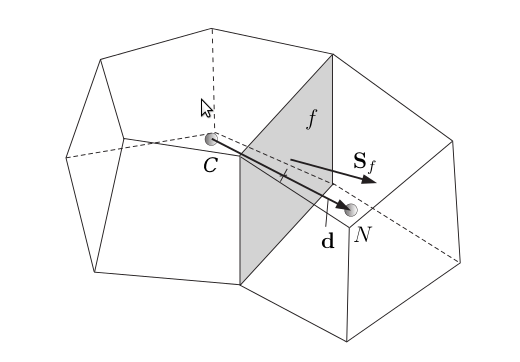
\includegraphics[scale=0.5]{twoCells}
			\caption{Схематическое изображение двух соседних ячеек}
			\label{fig:twoCells}
		\end{figure}
		\subsubsection*{Дискретизация уравнений}
		\addcontentsline{toc}{subsubsection}{Дискретизация уравнений}
		\begin{figure}[ht]
			\begin{minipage}{0.43\linewidth}
				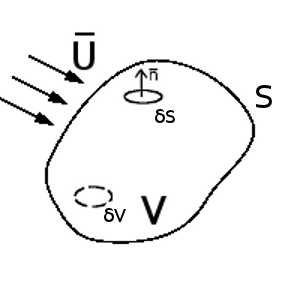
\includegraphics[scale=0.5]{controlVolume}
				\vspace{-2em}
				\caption{Контрольный объём}
				\label{fig:volume}
			\end{minipage}
			\hspace{-1em}
			\begin{minipage}{0.6\linewidth}
				\vspace{-2em}
				Пусть через контрольный объём $V$ \textit{(рисунок \ref{fig:volume})}, ограниченный контрольной поверхностью $S$, $\vec{\delta S} = \vec{n} \delta S$, проходит жидкость со скоростью $\vec{U}$. Выделим бесконечно малый объём $\delta V$. 
			\end{minipage}
		\end{figure}
		Рассмотрим скалярную величину $\Phi$ - плотность распределения некоторой физической величины на единицу массы. Тогда, с учётом того, что $\rho \delta V = \delta m$, в объёме $\delta V$ содержится $\rho \delta V \Phi$ этой физической величины. Уравнение сохранения для этой величины запишется, как
		\begin{equation}
			\frac{\partial}{\partial t} \int_V \rho \Phi \delta V + \oint_S \left( \rho \vec{U} \Phi + \vec{q}_{\Phi}  \right)\cdot \vec{\delta S} = \int_V \rho S_{\phi} \delta V,
			\label{transportEquation}
		\end{equation}
		где $S_{\Phi}$ - суммарная плотность источников, а $\vec{q}_{\Phi}$ -- дифузионный поток. Это уравнение применяется к каждому контрольному объёму. Задача заключается в сведении уравнения (\ref{transportEquation}) к процедуре алгебраического характера.
		
		Введём точку $C$ -- центр ячейки \textit(рисунок \ref{fig:twoCells}) и применим теорему о среднем к объёмному интегралу:
		\begin{figure}[h]
			\begin{minipage}{0.43\linewidth}
				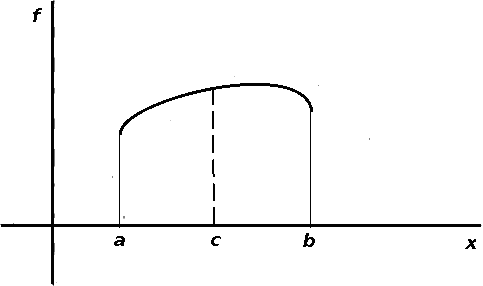
\includegraphics[scale=0.5]{meanValueTheorem}
				\label{fig:meanValueTheorem}
			\end{minipage}
			\hspace{-1em}
			\begin{minipage}{0.6\linewidth}
				\begin{equation}
					\int_a^b fdx \approx f(x_c) \cdot (b-a)
				\end{equation}
				\begin{equation}
					V \frac{\partial \left(\rho \Phi\right)_c}{\partial t} + \oint_S \left( \rho \vec{U} \Phi + \vec{q}_{\Phi}  \right)\cdot \vec{\delta S} = V \left( \rho S_{\Phi} \right)_c
				\end{equation}
				\vspace{2em}
			\end{minipage}
		\end{figure}
			\vspace{-1em}
					
			Пусть контрольная поверхность состоит из граней, то есть имеется огранённый объект. Тогда
			\begin{equation}
				\oint\left(\rho \vec{U} \Phi + \vec{q}_{\Phi} \right) \cdot \vec{\delta S} = \sum_f \int_{S_f} \left(\rho \vec{U} \Phi + \vec{q}_{\Phi} \right) \cdot \vec{\delta S},
			\end{equation}
			где $f$ -- номер грани.
			\begin{equation}
				\int_{S_f} \left(\rho \vec{U} \Phi + \vec{q}_{\Phi} \right) \cdot \vec{\delta S} \approx \left(\rho \vec{U} \Phi + \vec{q}_{\Phi} \right)_f \cdot \vec{S}_f,
			\end{equation}
			где индекс $f$ в выражении $\left(\rho \vec{U} \Phi  + \vec{q}_{\Phi}\right)_f$ означает, что это значение вычисляется в центре грани, а $\vec{S}_f = \vec{n} S_f$. В итоге мы получаем алгебраическое выражение
			\begin{equation}
				V\frac{\partial \left( \rho \Phi \right)_c}{\partial t} + \sum_f \left( \rho \vec{U} \Phi + \vec{q}_{\Phi} \right)_f \cdot \vec{S}_f = V \left( \rho S_{\Phi} \right)_c
			\end{equation}
		\subparagraph{Расчёт диффузионных потоков}
		\begin{equation}
			\int_V \nabla \cdot \left( \Gamma \nabla \Phi \right) \delta V = \int_S \vec{\delta S} \cdot (\Gamma \nabla \Phi) = \sum_f \Gamma_f \vec{S}_f \cdot (\nabla \Phi)_f
		\end{equation}
		\subparagraph{Расчёт ковективных потоков}
		\begin{equation}
			\int_V \nabla \cdot (\rho \vec{U} \Phi) \delta V = \int_S \vec{\delta S} \cdot (\rho \vec{U} \Phi) = \sum_f \vec{S}_f \cdot (\rho \vec{U})_f \Phi_f = \sum_f F \Phi_f
		\end{equation}
		Значение $\Phi_f$ на грани ячейки может быть определено с использованием различных схем:
		
		\textit{Центральная схема (CD)}
		\begin{equation}
		\Phi_f = \beta \Phi_N + (1-\beta)\Phi_C,
		\end{equation}
		где $\beta=\frac{\vec{|CM|}}{\vec{|CM|} + \vec{|NM|}}$ - коэффициент интерполяции, а точка $M$ -- центр грани $f$.
		
		Для коррекции на скошенность ячеек, когда центр грани $f$ не совпадает с пересечением грани $f$ и вектора $\vec{|CP|}$ (точка $M^{'}$), разложим $\Phi_f$ в ряд Тейлора в окрестности точки $M$ и удержим только первые два слагаемых:
		\begin{equation}
			\Phi_M = \Phi_{M^{'}} + \nabla \Phi_{M^{'}} \cdot \vec{M^{'}M} + O\left(\left(M-M^{'}\right)^2\right)
		\end{equation}
		
		\textit{Противопоточная схема (UD)}
		\begin{equation}
			\begin{aligned}
				\Phi_f = \Bigg\{	\begin{array}{l}
					\Phi_P, \quad \text{если } F \geq 0 \\
					\Phi_N, \quad \text{если } F < 0
				\end{array}
			\end{aligned}
		\end{equation}
		
		\textit{Смешанные схемы}
		\begin{equation}
			\Phi_f = \left(1-\gamma\right)(\Phi_f)_{UD} + \gamma (\Phi_f)_{CD},
		\end{equation}
		где коэффициент $\gamma$ меняется в зависимости от конкретной схемы.
		
		\subparagraph{Расчёт градиентов\\}
		
		    Значение градиента может быть вычислено двумя различными способами.
			
			\textit{Метод Гаусса}
			
			Первый способ -- использование достаточно простой формулы Гаусса:
			\begin{equation}
				\int_V \nabla \Phi \delta V = \int_S \vec{\delta S} \Phi = \sum_f \vec{S}_f \Phi_f
			\end{equation}
			
			\textit{Метод наименьших квадратов}
			
			Второй -- несколько более сложный метод наименьших квадратов, суть которого объясняется следующим образом: значение $\Phi$ в точке $C$ может быть экстраполировано в соседнюю ячейку с центром в точке $N$ с использованием градиента в точке $C$. Экстраполированное значение в точке $N$ сравнивается с актуальным значением в этой точке и рассчитывается ошибка в определении $\Phi$. Если мы теперь минимизируем сумму квадратов взвешенных ошибок во всех соседних ячейках по отношению к градиенту, значение градиента будет аппроксимировано достаточно точно. Таким образом, вычислив сначала значение тензора
			\begin{equation}
				\mathbf{G} = \sum_N \omega_N^2 (\vec{CN}\vec{CN}),
			\end{equation}
			где весовая функция $\omega = 1/\vec{|CN|}$, а индекс $N$ означает суммирование по всем соседним граням, мы сможем вычислить значение градиента в точке $C$:
			\begin{equation}
				(\nabla \Phi)_C = \sum_N \omega_N^2 \mathbf{G}^{-1} \cdot  (\Phi_N - \Phi_C).
			\end{equation}
	%Метод конечных объёмов

%Численное моделирование

\newpage
\section{Результаты}
\subsection{Валидация модели турбулентности с поправкой на кривизну линий тока}
\label{UDUCTComparison}
\newpage
\subsection{Постановка задачи}
  \begin{minipage}{0.6\textwidth}
    \captionof{table}{Геометрия фильтра}
			\begin{tabular}{l l}
				\hline
				\label{geometrytable}
				Диаметр цилиндра, $D$ & $0.205m$ \\
				Диаметр выходной трубы, $D_e$ & $0.5D$ \\
				Высота входного канала, $a$ & $0.5D$ \\
				Ширина входного канала, $b$ & $0.2D$ \\
				Длина выходной трубы, $h_e$ & $0.75D$ \\
				Полная высота фильтра, $H$ & $4.0D$ \\
				Высота цилиндра, $h$ & $1.5D$ \\
				Диаметр нижнего сечения, $B$ & $0.36D$ \\
				Высота пылесборника, $h_d$ & $0.25D$ \\
				Диаметр пылесборника, $D_d$ & $0.75D$ \\
			\end{tabular}
    \end{minipage}
    \hspace{1em}
  \begin{minipage}{0.35\textwidth}
    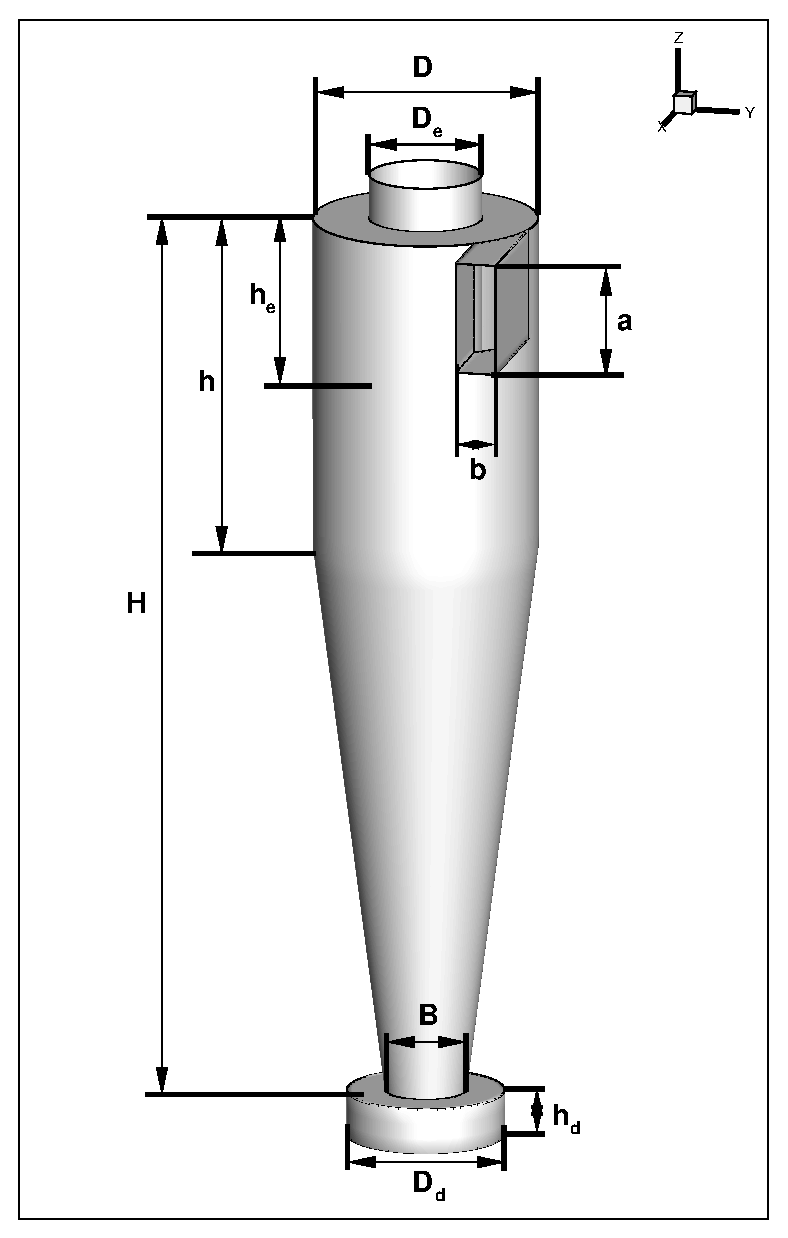
\includegraphics[scale=0.375]{Geometry}
				\captionof{figure}{Схема фильтра}
  \end{minipage}
%Решение

\clearpage
\newpage
%!TEX root = Dissertation.tex
\newpage
\thispagestyle{plain}
\bibliographystyle{unsrt}
\bibliography{dimbib}
\end{document}
